% Options for packages loaded elsewhere
\PassOptionsToPackage{unicode}{hyperref}
\PassOptionsToPackage{hyphens}{url}
%
\documentclass[
  11pt,
  ignorenonframetext,
  aspectratio=169]{beamer}
\usepackage{pgfpages}
\setbeamertemplate{caption}[numbered]
\setbeamertemplate{caption label separator}{: }
\setbeamercolor{caption name}{fg=normal text.fg}
\beamertemplatenavigationsymbolsempty
% Prevent slide breaks in the middle of a paragraph
\widowpenalties 1 10000
\raggedbottom
\setbeamertemplate{part page}{
  \centering
  \begin{beamercolorbox}[sep=16pt,center]{part title}
    \usebeamerfont{part title}\insertpart\par
  \end{beamercolorbox}
}
\setbeamertemplate{section page}{
  \centering
  \begin{beamercolorbox}[sep=12pt,center]{section title}
    \usebeamerfont{section title}\insertsection\par
  \end{beamercolorbox}
}
\setbeamertemplate{subsection page}{
  \centering
  \begin{beamercolorbox}[sep=8pt,center]{subsection title}
    \usebeamerfont{subsection title}\insertsubsection\par
  \end{beamercolorbox}
}
\AtBeginPart{
  \frame{\partpage}
}
\AtBeginSection{
  \ifbibliography
  \else
    \frame{\sectionpage}
  \fi
}
\AtBeginSubsection{
  \frame{\subsectionpage}
}
\usepackage{amsmath,amssymb}
\usepackage{iftex}
\ifPDFTeX
  \usepackage[T1]{fontenc}
  \usepackage[utf8]{inputenc}
  \usepackage{textcomp} % provide euro and other symbols
\else % if luatex or xetex
  \usepackage{unicode-math} % this also loads fontspec
  \defaultfontfeatures{Scale=MatchLowercase}
  \defaultfontfeatures[\rmfamily]{Ligatures=TeX,Scale=1}
\fi
\usepackage{lmodern}
\usetheme[]{default}
\usecolortheme{default}
\usefonttheme{structurebold}
\useinnertheme{rectangles}
\ifPDFTeX\else
  % xetex/luatex font selection
\fi
% Use upquote if available, for straight quotes in verbatim environments
\IfFileExists{upquote.sty}{\usepackage{upquote}}{}
\IfFileExists{microtype.sty}{% use microtype if available
  \usepackage[]{microtype}
  \UseMicrotypeSet[protrusion]{basicmath} % disable protrusion for tt fonts
}{}
\makeatletter
\@ifundefined{KOMAClassName}{% if non-KOMA class
  \IfFileExists{parskip.sty}{%
    \usepackage{parskip}
  }{% else
    \setlength{\parindent}{0pt}
    \setlength{\parskip}{6pt plus 2pt minus 1pt}}
}{% if KOMA class
  \KOMAoptions{parskip=half}}
\makeatother
\usepackage{xcolor}
\newif\ifbibliography
\usepackage{graphicx}
\makeatletter
\newsavebox\pandoc@box
\newcommand*\pandocbounded[1]{% scales image to fit in text height/width
  \sbox\pandoc@box{#1}%
  \Gscale@div\@tempa{\textheight}{\dimexpr\ht\pandoc@box+\dp\pandoc@box\relax}%
  \Gscale@div\@tempb{\linewidth}{\wd\pandoc@box}%
  \ifdim\@tempb\p@<\@tempa\p@\let\@tempa\@tempb\fi% select the smaller of both
  \ifdim\@tempa\p@<\p@\scalebox{\@tempa}{\usebox\pandoc@box}%
  \else\usebox{\pandoc@box}%
  \fi%
}
% Set default figure placement to htbp
\def\fps@figure{htbp}
\makeatother
\setlength{\emergencystretch}{3em} % prevent overfull lines
\providecommand{\tightlist}{%
  \setlength{\itemsep}{0pt}\setlength{\parskip}{0pt}}
\setcounter{secnumdepth}{-\maxdimen} % remove section numbering
\newcommand{\setfigheight}[1]{\setkeys{Gin}{height=#1,keepaspectratio}}
\newcommand{\setfigwidth}[1]{\setkeys{Gin}{width=#1,keepaspectratio}}
\newcommand{\setrelfigwidth}[1]{\setfigwidth{#1\csname textwidth\endcsname}}
\newcommand{\setrelfigheight}[1]{\setfigheight{#1\csname textheight\endcsname}}
\usepackage{tikz}
\usetikzlibrary{arrows.meta}
\usepackage{fontspec}
\setsansfont{Montserrat}
\logo{
\includegraphics[width=1.45\textwidth,height=1.02\textheight]{regularslide.pdf}}
% Additional colors
\definecolor{goldenrod}{rgb}{0.85,0.65,0.13}
\definecolor{silver}{gray}{0.75}
\definecolor{gray90}{gray}{0.9}
\definecolor{gray15}{gray}{0.15}

% Fit margins to the theme's logo
\setbeamersize
{
    text margin left=1cm,
    text margin right=1.4cm
}

% Title page
\defbeamertemplate*{title page}{customized}[1][]
{
\begin{picture}(0,0)
\put(-35.5,-153.5){
\includegraphics[width=16cm,height=9cm]{firstslide.pdf}}
\put(30,-28){\begin{minipage}{13cm}\begin{flushright}
\titlefont\color{white}
  \Huge{\inserttitle}\vspace{2pc}\par
  \normalsize\insertauthor\par
  \small\insertinstitute\vspace{.4pc}\par
  \small DRIConnect 2026 - \insertdate\par
  \end{flushright}
  \end{minipage}}
\end{picture}
}

% Section pages
\setbeamertemplate{section page}{
\begin{picture}(0,0)
\put(-36,-180){
\includegraphics[width=16.16cm,height=9.09cm]{sectionslide.pdf}}
\end{picture}
\vspace{2cm}\\
    \usebeamerfont{section title}\usebeamercolor[fg]{section title}\color{white}\titlefont\Huge\insertsection\textcolor{goldenrod}{.}
}

% Title on top of slides
\newfontfamily\titlefont{Ubuntu Light}
\setbeamertemplate{frametitle}{\ \\\vspace{2pt}\titlefont\Huge\color{gray15}\insertframetitle }

% Syntax-highlighted code blocks
\usepackage{tcolorbox}
%\renewenvironment{Shaded}{\begin{tcolorbox}[left=0pt,right=0pt,top=0pt,bottom=0pt,colframe=gray90,colback=gray90,arc=0pt]\small}{\end{tcolorbox}}

% Colors of third-level boxes
\setbeamercolor{structure}{fg=black,bg=goldenrod} % itemize, enumerate, etc
\setbeamercolor{alerted text}{fg=cyan!45!black}

% Slide number at the bottom left
\setbeamertemplate{footline}[text line]{%
  \parbox{\linewidth}{\vspace*{-14pt}\hspace*{-4cm}\titlefont{\large\color{silver}\ \ \ \insertframenumber}\hfill}}
\setbeamertemplate{navigation symbols}{}
\linespread{.9}

\usepackage{bookmark}
\IfFileExists{xurl.sty}{\usepackage{xurl}}{} % add URL line breaks if available
\urlstyle{same}
\hypersetup{
  pdftitle={The International HPC Summer School},
  pdfauthor={Ramses van Zon, Tania Tan},
  hidelinks,
  pdfcreator={LaTeX via pandoc}}

\title{The International HPC Summer School}
\author{Ramses van Zon, Tania Tan}
\date{May 26, 2026}

\begin{document}
\frame[plain]{\titlepage}

\begin{frame}{What is the IHPCSS?}
\phantomsection\label{what-is-the-ihpcss}
\pause

\begin{itemize}
\item
  The International High Performance Computing Summer School is an in-person, one-week, intensive training event held in June or July in different locations in the world since 2010.

  \pause
\item
  International partners like XSEDE (US), PRACE (EU) and RIKEN (Japan) select students with the potential to use and advance HPC in their respective fields.

  \pause
\item
  They pay for those students to attend, and also provide and fund instructors and staff.

  \pause
\item
  The event contains a unique mentoring component to help students navigate their careers in HPC.

  \pause
\item
  Compute Canada was a partner from 2014 until 2017, and SciNet from 2018 till 2023, and the Alliance from 2025 onwards.
\end{itemize}
\end{frame}

\begin{frame}{Alliance Pilot Project}
\phantomsection\label{alliance-pilot-project}
Tania?
\end{frame}

\begin{frame}{NTCC IHPCSS Working Group}
\phantomsection\label{ntcc-ihpcss-working-group}
\pause

\vspace{-3mm}

\begin{itemize}
\item
  Being a partner involves:

  \begin{itemize}
  \tightlist
  \item
    attending the international organization committee meetings
  \item
    being part of the program development
  \item
    running the selection process for Canadian applications
  \item
    inviting selected students, and
  \item
    supporting them at the event.
  \end{itemize}

  \pause
\item
  The Alliance delegated these to the National Training Coordination Council (NTCC).

  \pause
\item
  The Alliance requires a proposal for the event's funding, which the WG wrote.\\
  (It helps that the Alliance Training Coordinator is part of the WG).

  \pause
\item
  Finance and conditions on expenses were, handled by the Alliance in 2025, by SciNet in 2026.

  \pause
\item
  The latter required another proposal from SciNet to the Alliance.
\end{itemize}
\end{frame}

\begin{frame}{IHPCSS 2025: Lisbon, Portugal}
\phantomsection\label{ihpcss-2025-lisbon-portugal}
\begin{columns}[T]
\begin{column}{0.47\linewidth}\setlength{\parskip}{0.5\baselineskip}
\pandocbounded{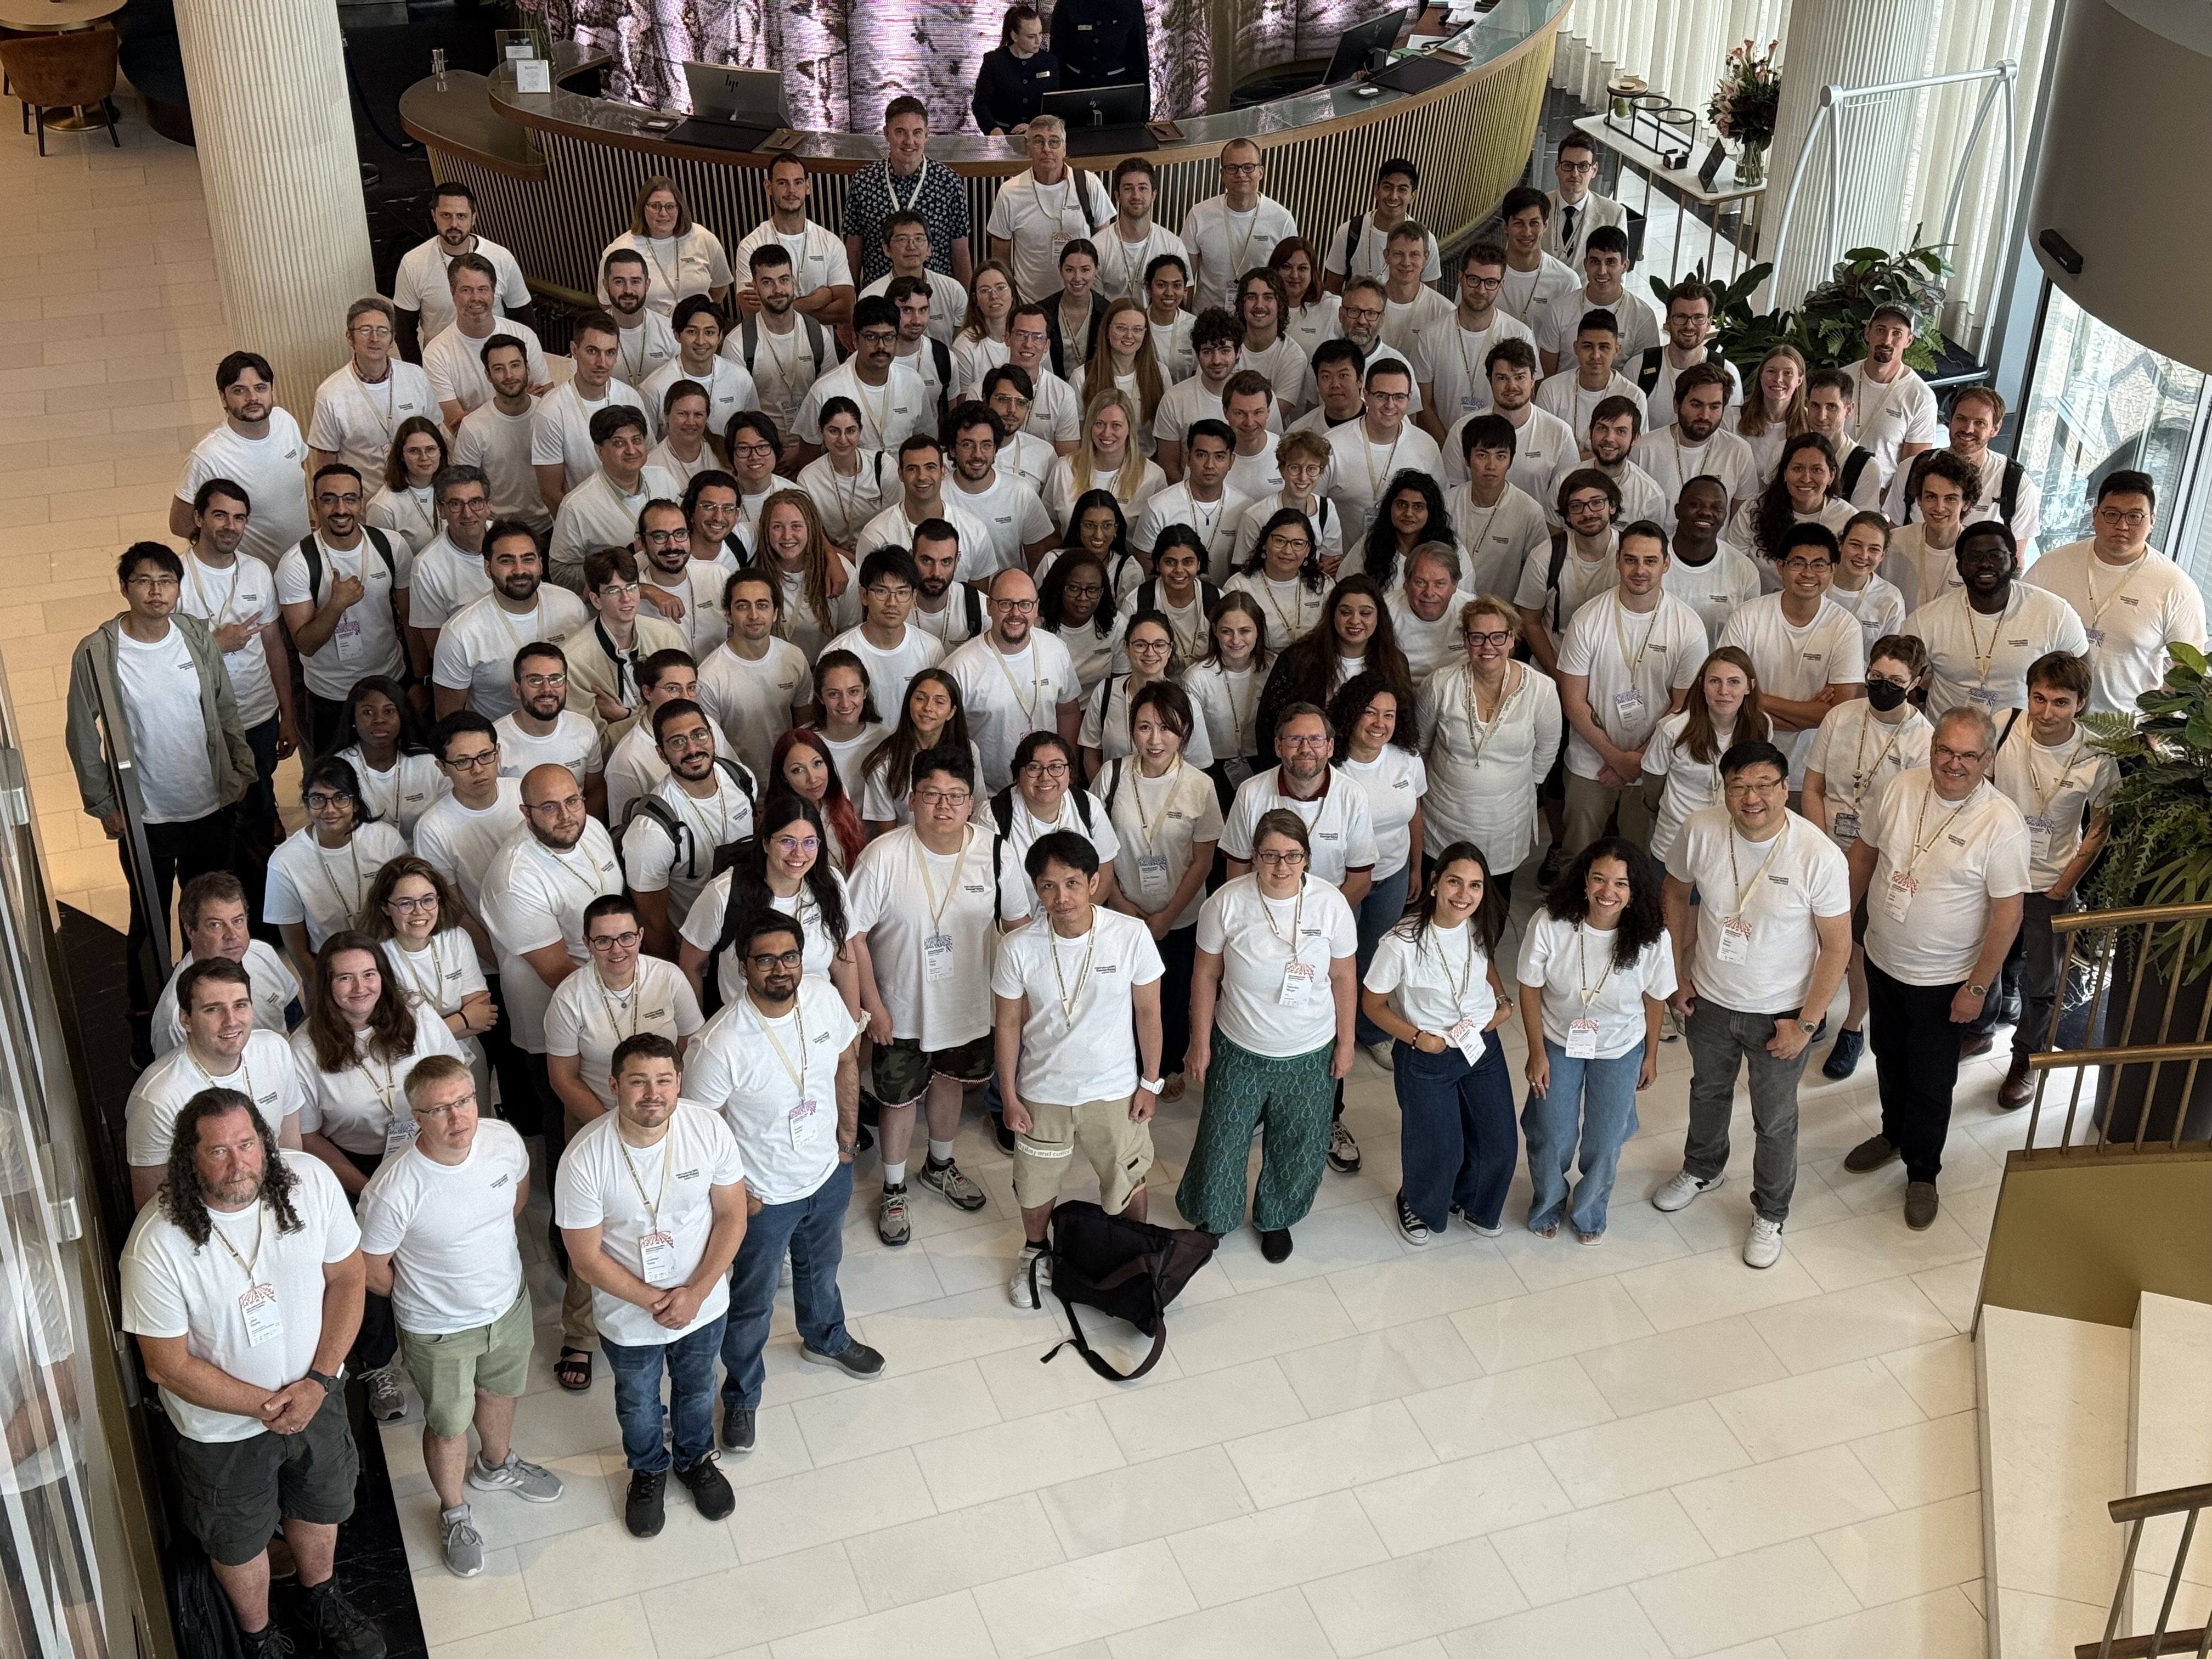
\includegraphics[keepaspectratio]{IHPCSS2025GroupPhoto.jpg}}
\end{column}

\begin{column}{0.47\linewidth}\setlength{\parskip}{0.5\baselineskip}
\textbf{\alert{\url{https://ss25.ihpcss.org}}}

\pause

\begin{itemize}
\item
  Canadian students applied: \textbf{137}

  \pause
\item
  Canadian students selected: \textbf{10}

  \pause
\item
  Returning mentor: \textbf{1}

  \pause
\item
  Instructors sent:\\
  Yohai Meiron, James Willis, and Ramses van Zon (paid by SciNet)

  \pause
\item
  IHPCSS Working group:\\
  Sarah Huber, Moïra Dion, Ramses van Zon, and Catherine Di Vita
\end{itemize}
\end{column}
\end{columns}

\pause

\small

\begin{itemize}
\tightlist
\item
  Reviewers: Sarah Huber, Moïra Dion, Yohai Meiron, Alex Razoumov, James Willis, Sarah Cameron-Pesant, Bruno Mundim, Vladimir Slavnic, Marco Saldarriaga, Chris Want, Jerry Li, Matthew Smith, Paul Preney, Chris Loken, Jane Fry
\end{itemize}

\vspace{\baselineskip}
\end{frame}

\begin{frame}{IHPCSS 2026: Perth, Australia}
\phantomsection\label{ihpcss-2026-perth-australia}
\begin{columns}[T]
\begin{column}{0.47\linewidth}\setlength{\parskip}{0.5\baselineskip}
\vspace{\baselineskip} \vspace{\baselineskip}

\pandocbounded{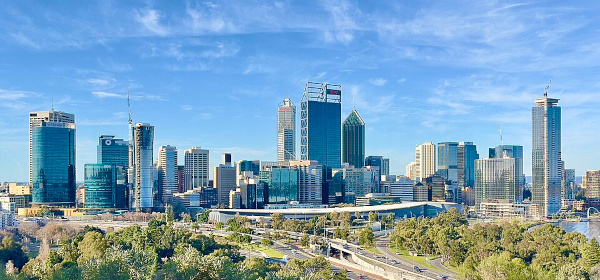
\includegraphics[keepaspectratio]{perth.jpg}}
\end{column}

\begin{column}{0.47\linewidth}\setlength{\parskip}{0.5\baselineskip}
\textbf{\alert{\url{https://ss26.ihpcss.org}}}

\pause

\begin{itemize}
\item
  Canadian students applied: \textbf{232}

  \pause
\item
  Canadian students selected: \textbf{10}

  \pause
\item
  Returning mentor: \textbf{1}

  \pause
\item
  Instructors to be sent:\\
  Sarah Huber, Alex Razoumov, Ramses van Zon

  \pause
\item
  IHPCSS Working group:\\
  Sarah Huber, Julie Faure-Lacroix, Ramses van Zon, and Tania Tan
\end{itemize}
\end{column}
\end{columns}

\pause

\small

\begin{itemize}
\tightlist
\item
  Reviewers: Yohai Meiron, Alex Razoumov, James Willis, Bruno Mundim, Vladimir Slavnic, Marco Saldarriaga, Chris Want, Jerry Li, Matthew Smith, Gurpreet Matharoo Chris Loken, Olivier Fisette, Ross Dickson, Patrick Mann
\end{itemize}

\vspace{\baselineskip}
\end{frame}

\begin{frame}{Evolving content}
\phantomsection\label{evolving-content}
\begin{itemize}
\item
  The main focus is and remains large scale HPC.

  \pause
\item
  The technical content is reviewed every year.

  \pause
\item
  The IHPCSS has changed significantly since the School was first run in 2010:

  \pause

  \begin{itemize}
  \tightlist
  \item
    GPU programming has become a standard component.
  \item
    The big data/machine learning/AI component is growing.
  \item
    There's even an Python for HPC session.
  \item
    But, on purpose, it will not become an AI conference.
  \item
    The mentoring component is unique and well-established.
  \end{itemize}

  \pause
\item
  Every year much effort is put into collecting feedback, understanding the skill landscape and adjusting the technical content.
\end{itemize}

\pause

\small

Scott Callaghan et al.~2025. Fifteen Years of International HPC Summer School. In PEARC '25, ACM, New York, NY, USA, Article 17, 1--8. \alert{\url{https://doi.org/10.1145/3708035.3736011}}
\end{frame}

\begin{frame}{Lessons Learned}
\phantomsection\label{lessons-learned}
\pause

\begin{itemize}
\item
  Budget needs fairly large margins to account for rising costs and unknown origins of participants.

  \pause
\item
  VISAs are always an uncertain issue; in 2025, two students could not make it because of delays in VISA appointments.

  \pause
\item
  The working group only needs to meet frequently in specific periods.

  \pause
\item
  We need more reviewers (or advertise less\ldots).

  \pause
\item
  Coordinating the finances between two organizations is painful and slow; best try to avoid.
\end{itemize}

\pause

\begin{block}{}\setlength{\parskip}{0.5\baselineskip}
\phantomsection\label{section}
\begin{itemize}
\item
  But it is worth it, there is a lot of demand.

  \pause
\item
  Hoping for a multi-year training strategy that includes this event!\\
  (so we may bring it to Canada?)
\end{itemize}
\end{block}
\end{frame}

\end{document}
